%=======================================================================



%=======================================================================


%====================================




%=======================================================================




%=======================================================================

%====================================

%=======================================================================


%=====================

%fig 3.3 
\begin{figure}
\centering
\begin{subfigure}{0.3\textwidth}
\centering
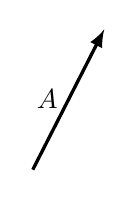
\begin{tikzpicture}
\draw[very thick, -latex] (0,0) -- (63:2) node[pos=0.5, left]{$\kvec{A}$};
\end{tikzpicture}
\caption{}
\end{subfigure}\hfill
\begin{subfigure}{0.3\textwidth}
\centering
\begin{tikzpicture}
\draw[-latex] (0,0) -- (0,2.25)coordinate(ytip) node[left]{$y$};
\draw[-latex] (0,0) -- (2,0)coordinate(xtip) node[below]{$x$};
\draw[-latex, very thick] (0,0) -- (1,2)coordinate(atip) node[pos=0.4,right]{$\kvec{A}$};
\draw[dashed](atip)--($(0,0)!(atip)!(xtip)$)coordinate(xi);
\draw[dashed](atip)--($(0,0)!(atip)!(ytip)$)coordinate(yi);
\draw (0.5,0) node[below]{$A_x$};
\draw (0,1.3) node[left]{$A_y$};
\draw (0.5,0) node[below]{$A_x$};
\end{tikzpicture}
\caption{}
\end{subfigure}\hfill
\begin{subfigure}{0.3\textwidth}
\centering
\begin{tikzpicture}
\draw [-latex] (0,0) -- (20:3)coordinate(xtip) node[below right]{$x'$};
\draw [-latex] (0,0) -- (110:3)coordinate(ytip) node[above right]{$y'$};
\draw[very thick, -latex] (0,0) -- (65:2.6)coordinate(a) node[pos=0.5, above left]{$\kvec{A}$};
\draw[dashed] (a) --  ($(0,0)!(a)!(xtip)$)coordinate(xi);
\draw[dashed] (a) --  ($(0,0)!(a)!(ytip)$)coordinate(yi);
\draw($(0,0)!0.5!(xi)$)node[below right]{$\kvec{A}_x'$};
\draw($(0,0)!0.5!(yi)$)node[left]{$\kvec{A}_y'$};
\end{tikzpicture}
\caption{}
\end{subfigure}
\caption{
(ا) سمتیہ \عددی{\kvec{A}}، (ب)  \عددی{xy} محدد سے لحاظ سے \عددی{\kvec{A}} کے اجزاء، (ج) \عددی{x'y'} محدد کے لحاظ سے \عددی{\kvec{A}} کے اجزاء
}
\label{
شکل_قواعد_سمتیہ_کے_اجزاء
}
\end{figure}

%=======================================================================

%fig 4.1
\begin{figure}
\centering
\begin{tikzpicture}
%\draw[help lines, thick,gray,step=1] (0,0) grid (12,12);
\draw[very thick, -latex] (6,6) -- (12,6);
\draw[dashed] (9,7.5) -- (9,4.5) -- (6,6);
\draw[dashed] (9,4.5) -- (10.5,6);
\draw[-latex] (6,6) -- (6,12) node[above]{$z$};
\draw[very thick] (6,6) -- (9,7.5) node[above]{$P$};
%\draw[-latex] (6,6) -- (135:6);
\end{tikzpicture}
\caption{}
\label{}
\end{figure}


%=============================================================

%fig 4.3

\begin{figure}
\centering
\begin{tikzpicture}
\pgfmathsetmacro{\r}{1.5}
\pgfmathsetmacro{\ra}{1.5-3/72}
\pgfmathsetmacro{\ang}{30}
\draw (0,0) circle (\r);
\draw[-latex] (0,0) node[circle,fill,inner sep=1.5pt]{} node[left]{$+e$} node[below left]{\RL{(پروٹان)}} -- (\ang:\ra) node[right]{$-e$} node[below right,xshift=0.4em]{\RL{(الیکٹران)}} node[pos=0.5, above]{$r$}node[circle,fill,inner sep=1.5pt]{};
\end{tikzpicture}
\caption{
ہائیڈروجن  جوہر
}
\label{
شکل_تین_ابعادی_ہائیڈروجن_جوہر
}
\end{figure}



%===================================================

%fig 4.11

\begin{figure}
\centering
\begin{tikzpicture}
\pgfmathsetmacro{\ang}{30}
\pgfmathsetmacro{\angA}{180-\ang}
\draw[-latex] (0,0) -- (1,0) node[below]{$y$};
\draw[-latex] (0,0) -- (0,1) node[left]{$z$};
\draw[-latex] (0,0) -- (-0.5,-0.5) node[below]{$x$};
\draw (1.5,0) -- (4,0) to [out=0,in=-\angA] ++ (1,0.3) --++ (\ang:2) node[right]{\RL{ہم میدان چکر}};
\draw (4,0) to [out=0,in=\angA] ++ (1,-0.3) --++ (-\ang:2)  node[right]{\RL{مخالف میدان چکر}};
\draw[fill=gray] (3.5,0.25) rectangle ++ (1,0.5);
\draw[fill=gray] (3.5,-0.25) rectangle ++ (1,-0.5);
\draw (4,-0.75) node[below]{\RL{مقناطیس}};
\draw[-latex] (1.5,0.25) --++ (1,0);
\draw[-latex] (5.5,0.85) --++ (\ang:1);
\draw[-latex] (5.5,-0.85) --++ (-\ang:1);
\end{tikzpicture}
\caption{
شٹرن و گرلاخ آلہ
}
\label{
شکل_تین_ابعادی_شٹرن_گرلاخ_آلہ
}
\end{figure}

%================================================

%fig 5.1 (p221)
\begin{figure}
\centering
\begin{subfigure}{0.35\textwidth} 
\centering
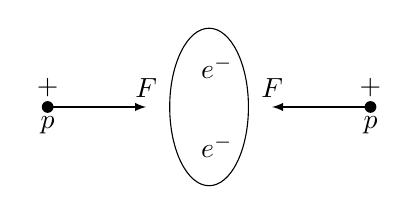
\begin{tikzpicture}
\draw (0,0) ellipse (0.5cm and 1cm);
\draw (0.1,0.5) node[]{$e^-$};
\draw (0.1,-0.5) node[]{$e^-$};
\draw[latex-] (-0.8,0) node[above]{$F$} --++ (-1.25,0) node[circle, fill, inner sep=1.5pt]{} node[below]{$p$} node[above]{$+$};
\draw[latex-] (0.8,0) node[above]{$F$} --++ (1.25,0) node[circle, fill, inner sep=1.5pt]{} node[below]{$p$} node[above]{$+$};
\end{tikzpicture}
\caption{}
\end{subfigure}\hfill
\begin{subfigure}{0.55\textwidth} 
\centering
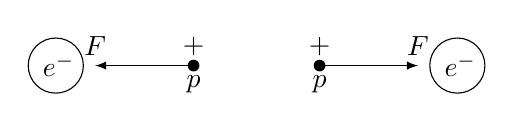
\begin{tikzpicture}
\draw[-latex] (-0.8,0) node[circle, fill, inner sep=1.5pt]{} node[below]{$p$} node[above]{$+$} --++ (-1.25,0) node[above]{$F$};
\draw[-latex] (0.8,0) node[circle, fill, inner sep=1.5pt]{} node[below]{$p$} node[above]{$+$} --++ (1.25,0) node[above]{$F$};
\draw (-0.8, 0) ++ (-1.25,0) ++ (-0.5,0) node[xshift=0.25ex]{$e^-$} circle (0.35);
\draw (0.8, 0) ++ (1.25,0) ++ (0.5,0) node[xshift=0.25ex]{$e^-$} circle (0.35);
\end{tikzpicture}
\caption{}
\end{subfigure}
\caption{
شریک گرفتی بندھ کی نقشہ کشی: (ا)  تشاکل تنظیم قوت کشش پیدا کرتی ہے، (ب)  خلاف تشاکل تنظیم قوت دفع پیدا کرتی ہے۔
}
\label{
شکل_دو_اجزا_تشاکل_اور_خلاف_تشاکل_تنظیم
}
\end{figure}

%===============================
%Table 5.1 Page 229.
\begin{table}
\caption{
دوری جدول  کے اولین چار  قطاروں کی الیکٹران تنظیم
}
\label{
جدول_یکساں_دوری_جدول_الیکٹران_تنظیم
}
%\renewcommand{\arraystretch}{1.5}
\begin{tabular}{rlll}
\toprule
Z & عنصر &\multicolumn{2}{l}{
تنظیم
\quad\quad\quad
}\\
\midrule
1 & \ce{H} & $(1s)$ & $^2S_{1/2}$\\
2 & \ce{He} & $(1s)^2$ & $^1S_{0}$\\
\midrule
3 & \ce{Li} & $(\ce{He})(2s)$ & $^2S_{1/2}$\\
4 & \ce{Be} & $(\ce{He})(2s)^2$ & $^1S_{0}$\\
\midrule
5 & \ce{B} & $(\ce{He})(2s)^2(2p)$ & $^2P_{1/2}$\\
6 & \ce{C} & $(\ce{He})(2s)^2(2p)^2$ & $^3P_{0}$\\
7 & \ce{N} & $(\ce{He})(2s)^2(2p)^3$ & $^4S_{3/2}$\\
8 & \ce{O} & $(\ce{He})(2s)^2(2p)^4$ & $^3P_{2}$\\
9 & \ce{F} & $(\ce{He})(2s)^2(2p)^5$ & $^2P_{3/2}$\\
10 & \ce{Ne} & $(\ce{He})(2s)^2(2p)^6$ & $^1S_{0}$\\
\midrule
11 & \ce{Na} & $(\ce{Ne})(3s)$ & $^2S_{1/2}$\\
12 & \ce{Mg} & $(\ce{Ne})(3s)^2$ & $^1S_{0}$\\
\midrule
13 & \ce{Al} & $(\ce{Ne})(3s)^2(3p)$ & $^2P_{1/2}$\\
14 & \ce{Si} & $(\ce{Ne})(3s)^2(3p)^2$    &    $^3P_{0}$\\
15 & \ce{P} & $(\ce{Ne})(3s)^2(3p)^3$    &    $^4S_{3/2}$\\
16 & \ce{S} & $(\ce{Ne})(3s)^2(3p)^4$    &    $^3P_{2}$\\
17 & \ce{Cl} & $(\ce{Ne})(3s)^2(3p)^5$    &    $^2P_{3/2}$\\
18 & \ce{Ar} & $(\ce{Ne})(3s)^2(3p)^6$    &    $^1S_{0}$\\
\midrule
19 & \ce{K} & $(\ce{Ar})(4s)$    &    $^2S_{1/2}$\\
20 & \ce{Ca} & $(\ce{Ar})(4s)^2$    &    $^1S_{0}$\\
\midrule
21 & \ce{Sc} & $(\ce{Ar})(4s)^2(3d)$    &    $^2D_{3/2}$\\
22 & \ce{Ti} & $(\ce{Ar})(4s)^2(3d)^2$    &    $^3F_{2}$\\
23 & \ce{V} & $(\ce{Ar})(4s)^2(3d)^3$    &    $^4F_{3/2}$\\
24 & \ce{Cr} & $(\ce{Ar})(4s)(3d)^5$    &    $^7S_{3}$\\
25 & \ce{Mn} & $(\ce{Ar})(4s)^2(3d)^5$    &    $^6S_{5/2}$\\
26 & \ce{Fe} & $(\ce{Ar})(4s)^2(3d)^6$    &    $^5D_{4}$\\
27 & \ce{Co} & $(\ce{Ar})(4s)^2(3d)^7$    &    $^4F_{9/2}$\\
28 & \ce{Ni} & $(\ce{Ar})(4s)^2(3d)^8$    &    $^3F_{4}$\\
29 & \ce{Cu} & $(\ce{Ar})(4s)(3d)^{10}$    &    $^2S_{1/2}$\\
30 & \ce{Zn} & $(\ce{Ar})(4s)^2(3d)^{10}$    &    $^1S_{0}$\\
\midrule
31 & \ce{Ga} & $(\ce{Ar})(4s)^2(3d)^{10}(4p)$    &    $^2P_{1/2}$\\
32 & \ce{Ge} & $(\ce{Ar})(4s)^2(3d)^{10}(4p)^2$    &    $^3P_{0}$\\
33 & \ce{As} & $(\ce{Ar})(4s)^2(3d)^{10}(4p)^3$    &    $^4S_{3/2}$\\
34 & \ce{Se} & $(\ce{Ar})(4s)^2(3d)^{10}(4p)^4$    &    $^3P_{2}$\\
35 & \ce{Br} & $(\ce{Ar})(4s)^2(3d)^{10}(4p)^5$    &    $^2P_{3/2}$\\
36 & \ce{Kr} & $(\ce{Ar})(4s)^2(3d)^{10}(4p)^6$    &    $^1S_{0}$\\
\bottomrule
\end{tabular}
\end{table}

%====================


%fig 5.3 Page 232

\begin{figure}
\centering 
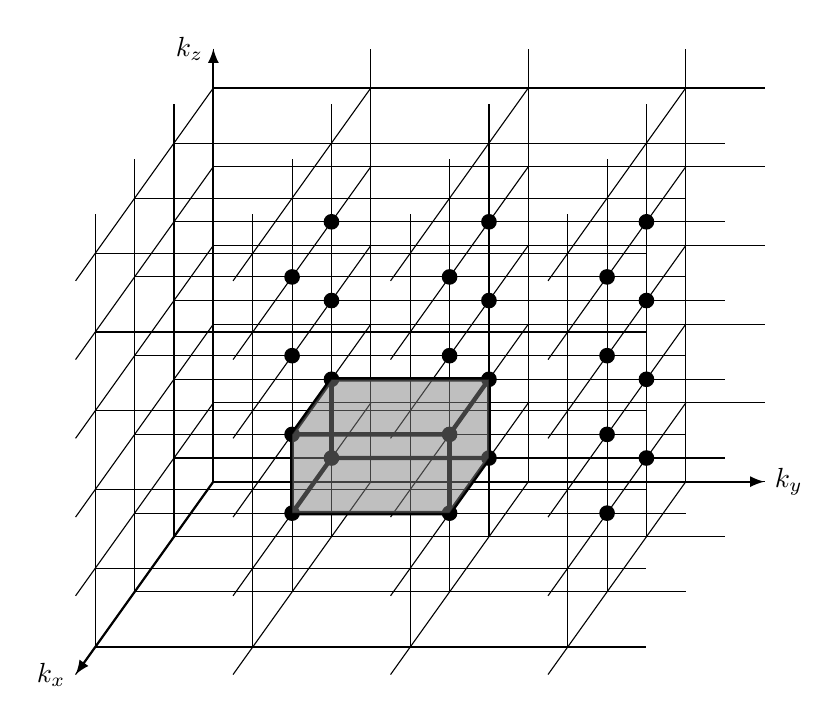
\begin{tikzpicture}[x={(-0.5cm,-0.70cm)}, y={(2cm,0cm)}, z={(0cm,1cm)}]
\draw[-latex, thick] (0,0,0) -- (3.5,0,0) node[left]{$k_x$};
\draw[-latex, thick] (0,0,0) -- (0,3.5,0) node[right]{$k_y$};
\draw[-latex, thick] (0,0,0) -- (0,0,5.5) node[left]{$k_z$};
\foreach \x in {0,1,2,3}{\draw (\x,0,0) -- (\x, 3.5, 0)  (\x,0,1) -- (\x,3.5,1) (\x,0,2) -- (\x,3.5,2)  (\x,0,3) -- (\x,3.5,3)  (\x,0,4) -- (\x,3.5,4) (\x,0,5) -- (\x,3.5,5)  ;}
\foreach \y in {0,1,2,3}{\draw (0,\y,0) -- (3.5, \y, 0)  (0,\y,1) -- (3.5, \y, 1) (0,\y,2) -- (3.5, \y, 2)  (0,\y,3) -- (3.5, \y, 3) (0,\y,4) -- (3.5, \y, 4) (0,\y,5) -- (3.5, \y, 5) ;}
\foreach \x in {0,1,2,3}{\draw (\x,0,0) -- (\x, 0,5.5)   (\x,1,0) -- (\x, 1,5.5)   (\x,2,0) -- (\x, 2,5.5)   (\x,3,0) -- (\x, 3,5.5)  ;}
\draw[ultra thick] (1,1,1) -- (2,1,1) -- (2,2,1) -- (1,2,1) -- (1,1,1);
\draw[ultra thick] (1,1,2) -- (2,1,2) -- (2,2,2) -- (1,2,2) -- (1,1,2);
\draw[ultra thick] (1,1,1) node[circle, fill, inner sep=2pt]{} -- (1,1,2) node[circle, fill, inner sep=2pt]{} (2,1,1) node[circle, fill, inner sep=2pt]{} -- (2,1,2) node[circle, fill, inner sep=2pt]{} (2,2,1) node[circle, fill, inner sep=2pt]{} -- (2,2,2) node[circle, fill, inner sep=2pt]{} (1,2,1) node[circle, fill, inner sep=2pt]{} -- (1,2,2) node[circle, fill, inner sep=2pt]{};
\draw[fill=gray, opacity=0.5] (1,1,2) -- (2,1,2) -- (2,1,1) -- (2,2,1) -- (1,2,1) -- (1,2,2) -- (1,1,2);
\foreach \z in {1,2,3,4} {\draw (1,3,\z) node[circle, fill, inner sep=2pt]{} (2,3,\z) node[circle, fill, inner sep=2pt]{};}
\foreach \z in {3,4} {\draw (1,1,\z) node[circle, fill, inner sep=2pt]{} (2,1,\z) node[circle, fill, inner sep=2pt]{} (1,2,\z) node[circle, fill, inner sep=2pt]{} (2,2,\z) node[circle, fill, inner sep=2pt]{};}
\end{tikzpicture}
\caption{
آزاد الیکٹران گیس۔ جال کا ہر نقطہ تقاطع ایک ساکن حال کو ظاہر کرتا ہے۔ ایک "ڈبا" کو سیاح دکھایا گیا ہے۔ ایک ڈبہ  کے لئے ایک حال پایا جاتا ہے۔
}
\label{
شکل_یکساں_ایک_ڈبا_ایک_حال
}
\end{figure}

%===================

\begin{figure}
\centering
\begin{tikzpicture}[x={(-0.5cm,-0.5cm)},y={(1cm,0cm)},z={(0cm,1cm)}]
%\pgfmathsetseed{1}
\pgfmathsetmacro{\kr}{2.75}
\pgfmathsetmacro{\krd}{\kr+0.3}
\pgfmathsetmacro{\kphi}{60}
%\pgfmathsetmacro{\ktheta}{45}
%
%axis
\draw[-stealth] (0,0,0)--(3.25,0,0)node[left]{$k_x$};
\draw[-stealth] (0,0,0)--(0,3.25,0)node[below]{$k_y$};
\draw[-stealth] (0,0,0)--(0,0,3.25)node[left]{$k_z$};
% r, phi , theta
\begin{scope}[canvas is xy plane at z=0]
\draw(\kr,0,0) arc (0:90:\kr);
\draw(\krd,0,0) arc (0:90:\krd);
\end{scope}
%
\begin{scope}[canvas is xz plane at y=0]
\draw(\kr,0,0) arc (0:90:\kr);
\draw(\krd,0,0) arc (0:90:\krd);
\end{scope}
%
\begin{scope}[canvas is yz plane at x=0]
\draw(\kr,0,0) arc (0:90:\kr);
\draw(\krd,0,0) arc (0:90:\krd);
\draw[-latex] (0,0,0)--++(30:\kr)node[pos=0.5,below]{$\kvec{k}$};
\draw[latex-] (30:\krd)--++(30:0.5)node[right]{$\dif k$};
\end{scope}
\end{tikzpicture}%
\caption{
 کروی پوست کا  \عددی{k} فضا میں ایک مثمن۔
}
\label{
شکل_یکساں_کروی_پوست_مثمن
}
\end{figure}

%======================

\begin{figure}
\centering
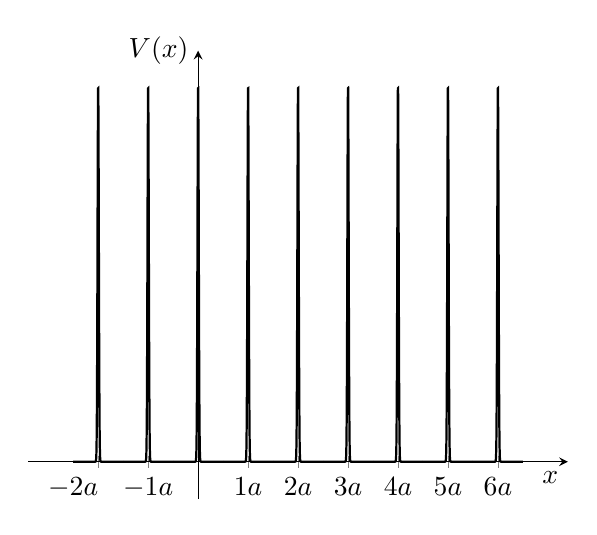
\begin{tikzpicture}
\begin{axis}[axis lines=middle,xlabel={$x$},ylabel={$V(x)$}, xtick={-2,-1,0,1,2,3,4,5,6},
 xticklabels={\llap{$-2a$} ,$-1a$, $0$,  $1a$, $2a$, $3a$, $4a$, $5a$, $6a$}, ytick={\empty}, ylabel style={at={(current axis.above origin)},anchor=east},xlabel style={at={(current axis.right of origin)},anchor=north east},enlargelimits]
\pgfmathsetmacro{\c}{-2}
\addplot [thick,domain=\c-0.5:\c+0.5,samples=200,]	{exp(-3000*(x-\c)^2)};
\pgfmathsetmacro{\c}{-1}
\addplot [thick,domain=\c-0.5:\c+0.5,samples=200,]	{exp(-3000*(x-\c)^2)};
\pgfmathsetmacro{\c}{0}
\addplot [thick,domain=\c-0.5:\c+0.5,samples=200,]	{exp(-3000*(x-\c)^2)};
\pgfmathsetmacro{\c}{1}
\addplot [thick,domain=\c-0.5:\c+0.5,samples=200,]	{exp(-3000*(x-\c)^2)};
\pgfmathsetmacro{\c}{2}
\addplot [thick,domain=\c-0.5:\c+0.5,samples=200,]	{exp(-3000*(x-\c)^2)};
\pgfmathsetmacro{\c}{3}
\addplot [thick,domain=\c-0.5:\c+0.5,samples=200,]	{exp(-3000*(x-\c)^2)};
\pgfmathsetmacro{\c}{4}
\addplot [thick,domain=\c-0.5:\c+0.5,samples=200,]	{exp(-3000*(x-\c)^2)};
\pgfmathsetmacro{\c}{5}
\addplot [thick,domain=\c-0.5:\c+0.5,samples=200,]	{exp(-3000*(x-\c)^2)};
\pgfmathsetmacro{\c}{6}
\addplot [thick,domain=\c-0.5:\c+0.5,samples=200,]	{exp(-3000*(x-\c)^2)};
\end{axis}
\end{tikzpicture}
\caption{
ڈیراک کنگھی۔ مساوات \حوالہء{5.57}
}
\label{شکل_یکساں_ڈیراک_کنگھی}
\end{figure}

%======================

\begin{figure}
\centering
\begin{tikzpicture}[declare function={f(\x)=cos(\x) + 10*180/(pi*\x)*sin(\x);}]
\begin{axis}[axis lines=middle,xlabel={$x$},ylabel={$V(x)$}, xtick={180,360,540,720},
 xticklabels={$\pi$,$2\pi$,$3\pi$,$4\pi$}, ytick={-1,1},yticklabels={$-1$,$1$}, ylabel style={at={(current axis.above origin)},anchor=east},xlabel style={at={(current axis.right of origin)},anchor=north east},enlargelimits]
\addplot[domain=130:900,samples=400, name path global=f]{f(x)};
\addplot[domain=0:900, name path global=xa] {1};
\addplot[domain=0:900, name path global=xb] {-1};
\end{axis}
\end{tikzpicture}
\caption{discarded, use the next figure instead}
\label{}
\end{figure}


%======================
%figure 5.6 pg 240

\begin{figure}
\centering
\begin{tikzpicture}[declare function={f(\x)=cos(\x) + 10*180/(pi*\x)*sin(\x);}]
%\addplot[domain=130:900,samples=400]{f(x)};
\draw (0,0) node[left]{$0$} -- (9,0) node[right]{$0$};
\draw [name path=xa] (0,1) node[left]{$1$} -- (9,1) node[right]{$1$};
\draw (0,2.75) -- (9,2.75);
\draw (0,-2.75) -- (9,-2.75);
\draw [name path=xb] (0,-1) node[left]{$-1$} -- (9,-1) node[right]{$-1$};
\draw (0,-2.75) node[below]{$0$} -- (0,2.75);
\draw (1.8,-2.75) node[below]{$\pi$} -- (1.8,2.75);
\draw [name path=ya] (3.6,-2.75) node[below]{$2\pi$} -- (3.6,2.75);
\draw [name path=yb] (5.4,-2.75) node[below]{$3\pi$} -- (5.4,2.75);
\draw [name path=yc] (7.2,-2.75) node[below]{$4\pi$} -- (7.2,2.75);
\draw [name path=yd] (9,-2.75) node[below]{$5\pi$} -- (9,2.75);
\draw[thick, domain=130:900,variable=\x,samples=400,name path=f] plot (\x/100,{cos(\x) + 10*180/(pi*\x)*sin(\x)});
\draw [fill=gray, opacity=0.5, name intersections={of={xa and f}}](intersection-1) --++ (0,-2) -- (1.8,-1) -- (1.8,1) -- (intersection-1);
\draw [fill=gray, opacity=0.5, name intersections={of={xb and f}}](intersection-2) --++ (0,2) -- (3.6,1) -- (3.6,-1) -- (intersection-2);
\draw [fill=gray, opacity=0.5, name intersections={of={xa and f}}](intersection-3) --++ (0,-2) -- (5.4,-1) -- (5.4,1) -- (intersection-3);
\draw [fill=gray, opacity=0.5, name intersections={of={xb and f}}](intersection-4) --++ (0,2) -- (7.2,1) -- (7.2,-1) -- (intersection-4);
\draw [fill=gray, opacity=0.5, name intersections={of={xa and f}}](intersection-5) --++ (0,-2) -- (9,-1) -- (9,1) -- (intersection-5);
\end{tikzpicture}
\caption{
تفاعل \عددی{f(z)}  (مساوات \حوالہء{5.66})  کو \عددی{\beta=10} کے لئے ترسیم کر کے اجازتی  پٹیاں  (سایہ دار)  دکھائی گئی ہیں  جن کے بیچ  ممنوعہ درز   (جہاں \عددی{\abs{f(z)}>1}  ہو گا)  پائے  جاتے ہیں۔
}
\label{
شکل_یکساں_اجازتی_ممنوعہ_پٹیاں
}
\end{figure}


%============================================

%fig 5.7 pg 240

\begin{figure}
\centering
\begin{tikzpicture}
\pgfmathsetmacro{\a}{1}
\pgfmathsetmacro{\c}{2.5}
\pgfmathsetmacro{\e}{3.9}
\draw[-stealth] (0,0) -- (0,5.5) node[left]{$E$};
\draw[] (0,0) -- (2,0) -- (2,4.5);
\foreach \y in{0,0.05,...,0.70}{\draw[thin](0,\y+\a) -- (2,\y+\a);}
\foreach \y in{0,0.05,...,1}{\draw[thin](0,\y+\c) -- (2,\y+\c);}
\foreach \y in{0,0.05,...,1.25}{\draw[thin](0,\y+\e) -- (2,\y+\e);}
\draw [decorate, decoration={brace,amplitude=5pt,mirror},xshift=4pt] (2,1) -- (2,1.7) node[midway,xshift=15pt]{پٹی};
\draw [decorate, decoration={brace,amplitude=5pt,mirror},xshift=4pt] (2,2.5) -- (2,3.5) node[midway,xshift=15pt]{پٹی};
\draw [decorate, decoration={brace,amplitude=5pt,mirror},xshift=4pt] (2,3.9) -- (2,5.15) node[midway,xshift=15pt]{پٹی};
\draw [decorate, decoration={brace,amplitude=5pt},xshift=-4pt] (0,0) -- (0,1) node[midway,xshift=-15pt]{درز};
\draw [decorate, decoration={brace,amplitude=5pt},xshift=-4pt] (0,1.7) -- (0,2.5) node[midway,xshift=-15pt]{درز};
\draw [decorate, decoration={brace,amplitude=5pt},xshift=-4pt] (0,3.5) -- (0,3.9) node[midway,xshift=-15pt]{درز};
\end{tikzpicture}
\caption{
دوری مخفیہ کی اجزاتی توانائیاں  بنیادی طور پر  استمراری پٹیاں پیدا کرتی ہیں۔
}
\label{
شکل_یکساں_دوری_مخفیہ_استمراری_پٹیاں
}
\end{figure}



%===================================================
%figure 5.8 pg 254

\begin{figure}
\centering
\pgfmathsetmacro{\T}{5}
\pgfmathsetmacro{\u}{1.5}
\pgfmathsetmacro{\k}{0.015}
\begin{tikzpicture}[declare function={f(\x)=1/(e^((\x-\u)/(\k*\T))+1);}]
\begin{axis}[axis lines=middle,xlabel={$\epsilon$},ylabel={$n(\epsilon)$}, xtick={\u},
 xticklabels={$E_F=\mu(0)$}, ytick={\empty},yticklabels={}, ylabel style={at={(current axis.above origin)},anchor=east},xlabel style={at={(current axis.right of origin)},anchor=north},enlargelimits]
\addplot[thin]coordinates{(0,1)(\u,1)(\u,0)} node[pos=0.65,pin={30:{$T=0$}}]{};
\addplot[thick,domain=0:2, smooth]{f(x)}node[pos=0.8,pin={30:{$T>0$}}]{};
\end{axis}
\end{tikzpicture}
\caption{فرمی و  ڈیراک تقسیم برائے \عددی{T=0} اور صفر سے کچھ  زیادہ \عددی{T} کے لئے۔}
\label{شکل_یکساں_فرمی_ڈیراک_تقسیم}
\end{figure}


%===================================================
%figure 5.9 pg 257

\begin{figure}
\centering
\pgfmathsetmacro{\k}{1/30}
\pgfmathsetmacro{\h}{1}
\begin{tikzpicture}[declare function={f(\x,\T)=0.09817*\x^3/(e^(4.8017956*\x/(\T))-1);}]
\begin{axis}[axis lines=middle,xlabel={$f\,[\SI{e14}{\hertz}]$},ylabel={$\rho(\omega)\,[\SI{e-15}{\joule\per\meter\cubed\per\hertz}]$}, xtick={2,4,6,8},, ytick={\empty},, ylabel style={at={(current axis.above origin)},anchor=east},ylabel style={xshift=-1em,rotate=90,},xlabel style={at={(current axis.right of origin)},anchor=north},enlargelimits]
\addplot[thick,domain=0:9, smooth]{f(x,2)}node[pos=0.3,above]{$\SI{2000}{\kelvin}$};
\addplot[thick,domain=0:9, smooth]{f(x,4)}node[pos=0.5,above right]{$\SI{4000}{\kelvin}$};
\addplot[thick,domain=0:9, smooth]{f(x,6)}node[pos=0.6,above right]{$\SI{6000}{\kelvin}$};
\addplot[dashed,gray]coordinates{(4,0)(4,0.3)};
\addplot[dashed,gray]coordinates{(8,0)(8,0.3)};
\addplot[<->]coordinates{(4,0.28)(8,0.28)}node[pos=0.5,fill=white]{\RL{بصری خطہ}};
\end{axis}
\end{tikzpicture}
\caption{
سیاہ جسمی   اخراج کے لئے کلیہ پلانک، مساوات \حوالہء{5.113}
}
\label{شکل_یکساں_فرمی_ڈیراک_تقسیم}
\end{figure}


%===================================

%fig 6.1 pg 262

\begin{figure}
\centering
\begin{tikzpicture}
\fill[path fading=west,color=lgray] (-0.25,0) rectangle (0,3.75);
\fill[path fading=east,color=lgray] (5,0) rectangle (5.25,3.75);
\draw[-stealth] (-0.5,0) -- (5.75,0)node[below]{$x$};
\draw[-stealth] (0,-0.25) -- (0,4)node[left]{$V(x)$};
\draw[very thick](0,3.75) -- (0,0) -- (3,0) to [out=30,in=180](3.5,0.5) to [out=0,in=150](4,0) -- (5,0)node[below]{$a$} -- (5,3.75);
\end{tikzpicture}
\caption{
لامتناہی چکور کنواں میں معمولی اضطراب
}
\label{
شکل_غیر_تابع_اضطراب_چکور_معمولی
}
\end{figure}


%===================================

%fig 6.2 pg 264

\begin{figure}
\centering
\begin{tikzpicture}
\fill[path fading=west,color=lgray] (-0.25,0) rectangle (0,3.75);
\fill[path fading=east,color=lgray] (5,0) node[below,black]{$a$} rectangle (5.25,3.75);
\draw[-stealth] (-0.5,0) -- (5.75,0)node[below]{$x$};
\draw[-stealth] (0,-0.25) -- (0,4)node[left]{$V(x)$};
\draw[very thick](0,3.75) -- (0,0.5)node[left]{$V_0$} -- (5,0.5) -- (5,3.75);
\end{tikzpicture}
\caption{
پورے کنواں میں مستقل اضطراب
}
\label{
شکل_غیر_تابع_اضطراب_چکور_مستقل_اضطراب
}
\end{figure}


%===================================

%fig 6.3 pg 265

\begin{figure}
\centering
\begin{tikzpicture}
\fill[path fading=west,color=lgray] (-0.25,0) rectangle (0,3.75);
\fill[path fading=east,color=lgray] (5,0) rectangle (5.25,3.75);
\draw[-stealth] (-0.5,0) -- (5.75,0)node[below]{$x$};
\draw[-stealth] (0,-0.25) -- (0,4)node[left]{$V(x)$};
\draw[very thick](0,3.75) -- (0,0.5)node[left]{$V_0$} -- (2.5,0.5) -- (2.5,0)node[below]{$\tfrac{a}{2}$} -- (5,0)node[below,black]{$a$} -- (5,3.75);
\end{tikzpicture}
\caption{
نصف  کنواں میں مستقل اضطراب
}
\label{
شکل_غیر_تابع_اضطراب_نصف_چکور_مستقل_اضطراب
}
\end{figure}



%===================================

%fig 6.4 pg 270

\begin{figure}
\centering
\begin{tikzpicture}
\draw[-stealth] (0,0) -- (6,0) node[below]{$\lambda$};
\draw[-stealth] (0,0) -- (0,4) node[left]{$E$};
\draw[thick] (0,2) to [out = 0, in=-140] (5,3.75);
\draw[thick] (0,2)node[left]{$E_0$} to [out = 0, in=140] (5,0.25);
\draw[dashed] (5,0) node[below]{$1$} -- (5, 4);
\end{tikzpicture}
\caption{
انحطاط کا خاتمہ بذریعہ اضطراب
}
\label{
شکل_غیر_تابع_اضطراب_اختتام_انحطاط
}
\end{figure}


%===================================

%fig 6.5 pg 275

\begin{figure}
\centering
\begin{tikzpicture}[x={(-0.5cm,-0.5cm)}, y={(1cm,0cm)},z={(0cm,1cm)}]
\pgfmathsetmacro{\a}{2.5}
\pgfmathsetmacro{\b}{2.5}
\pgfmathsetmacro{\c}{2.5}
\pgfmathsetmacro{\d}{\a/2}
\pgfmathsetmacro{\e}{\b/2}
\pgfmathsetmacro{\f}{\c}
\fill[lgray] (0,0,\f) -- (\d,0,\f) -- (\d,0,0) -- (\d,\e,0) -- (0,\e,0) -- (0,\e,\f) -- (0,0,\f);
\draw[-stealth] (0,0,0) -- (3.5,0,0) node[left]{$x$};
\draw[-stealth] (0,0,0) -- (0,4,0) node[below]{$y$};
\draw[-stealth] (0,0,0) -- (0,0,3.25) node[left]{$z$};
\draw[thick] (0,0,0) -- (\a,0,0)node[below]{$a$} -- (\a,\b,0) -- (0,\b,0)node[below]{$a$} -- (0,0,0);
\draw[thick] (0,0,\c) -- (\a,0,\c) -- (\a,\b,\c) -- (0,\b,\c) -- (0,0,\c);
\draw[thick] (0,0,0) -- (0,0,\c);
\draw[thick] (\a,0,0) -- (\a,0,\c);
\draw[thick] (\a,\b,0) -- (\a,\b,\c);
\draw[thick] (0,\b,0) -- (0,\b,\c);
\draw[thick] (0,0,0) -- (\d,0,0)  -- (\d,\e,0) -- (0,\e,0)  -- (0,0,0);
\draw[thick] (0,0,\f) -- (\d,0,\f) node[left, yshift=0.25em]{$a/2$} -- (\d,\e,\f) -- (0,\e,\f) node[above]{$a/2$} -- (0,0,\f) node[above right]{$a$};
\draw[thick] (0,0,0) -- (0,0,\f);
\draw[thick] (\d,0,0) -- (\d,0,\f);
\draw[thick] (\d,\e,0) -- (\d,\e,\f);
\draw[thick] (0,\e,0) -- (0,\e,\f);
\end{tikzpicture}
\caption{
سایہ دار خطہ میں مخفیہ کو اضطراب مقدار \عددی{V_0} بڑھاتا ہے۔
}
\label{
شکل_غیر_تابع_اضطراب_مخفیہ_بڑھنا_چکور_نما
}
\end{figure}



%===================================

%fig 6.6 pg 277

\begin{figure}
\centering
\begin{tikzpicture}
\draw[-stealth] (0,0) -- (6,0) node[below]{$\lambda$};
\draw[-stealth] (0,0) -- (0,4) node[left]{$E_1(\lambda)$};
\draw[thick] (0,1) node[left]{$E_1^0$} -- (5,1.5) node[right]{$E_1^0 + \lambda (1-k) \tfrac{V_0}{4}$};
\draw[thick] (0,1) -- (5,2.5) node[right]{$E_1^0 + \lambda \tfrac{V_0}{4}$};
\draw[thick] (0,1) -- (5,3.5)  node[right]{$E_1^0 + \lambda (1+k) \tfrac{V_0}{4}$};
\draw[dashed] (5,0) node[below]{$1$} -- (5, 4);
\end{tikzpicture}
\caption{
انحطاط کا اختتام (برائے مثال \حوالہء{6.39})۔
}
\label{
شکل_غیر_تابع_اضطراب_انحطاط_اختتام_مثال
}
\end{figure}

%===================================

%fig 6.7 pg 283

\begin{figure}
\centering
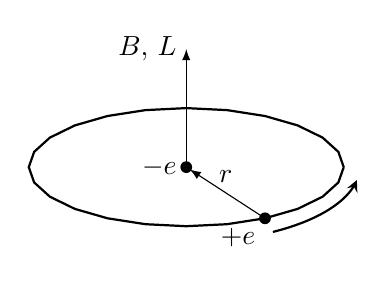
\begin{tikzpicture}[declare function={f(\x)=\ra*cos(\x) +\rb*sin(\x);}]
\pgfmathsetmacro{\ra}{2}
\pgfmathsetmacro{\rb}{0.75}
\pgfmathsetmacro{\rc}{\ra+0.2}
\pgfmathsetmacro{\rd}{\rb+0.2}
\draw[thick,domain=0:360]plot({\ra*cos(\x)},{\rb*sin(\x)});
\draw [-latex] (0,0) node[left]{$-e$} node[fill=black, circle, inner sep=1.5pt]{} -- (0,1.5) node[left]{$\kvec{B}, \, \kvec{L}$};
\draw [latex-,shorten <=1.5pt] (0,0) -- ({\ra*cos(300)},{\rb*sin(300)}) node[pos=0.5,above]{$r$} node[fill=black, circle, inner sep=1.5pt]{} node[below left]{$+e$};
\draw[-stealth,thick,domain=300:350]plot({\rc*cos(\x)},{\rd*sin(\x)});
\end{tikzpicture}
\caption{
الیکٹران کے نقطہ نظر سے ہائیڈروجن جوہر۔
}
\label{
شکل_غیر_تابع_اضطراب_جوہر_الیکٹران_نقطہ_نظر
}
\end{figure}

%===================================

%fig 6.8 pg 284

\begin{figure}
\centering
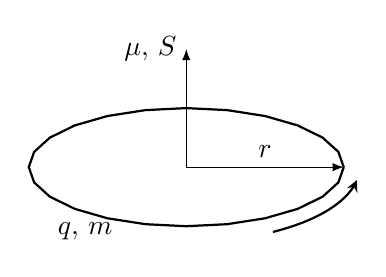
\begin{tikzpicture}[declare function={f(\x)=\ra*cos(\x) +\rb*sin(\x);}]
\pgfmathsetmacro{\ra}{2}
\pgfmathsetmacro{\rb}{0.75}
\pgfmathsetmacro{\rc}{\ra+0.2}
\pgfmathsetmacro{\rd}{\rb+0.2}
\draw[thick,domain=0:360]plot({\ra*cos(\x)},{\rb*sin(\x)});
\draw [-latex] (0,0) -- (0,1.5) node[left]{$\kvec{\mu}, \, \kvec{S}$};
\draw [-latex] (0,0) -- ({\ra*cos(0)},{\rb*sin(0)}) node[pos=0.5,above]{$r$};
\draw[-stealth,thick,domain=300:350]plot({\rc*cos(\x)},{\rd*sin(\x)});
\draw []  ({\ra*cos(230)},{\rb*sin(230)}) node[below]{$q,\, m$};
\end{tikzpicture}
\caption{
بار کا چھلا جو اپنے محور کے گرد گھوم رہا ہے۔
}
\label{
شکل_غیر_تابع_اضطراب_جوہر_الیکٹران_نقطہ_نظر
}
\end{figure}


%===================================

%fig 6.10 pg 290

\begin{figure}
\centering
\pgfmathsetmacro{\ra}{2}
\pgfmathsetmacro{\rb}{0.75}
\begin{tikzpicture}[declare function={f(\x)=\ra*cos(\x); g(\x)=\rb*sin(\x);}]
\draw[rotate around={-45:(0,0)}, domain=0:360] plot ({f(\x)},{g(\x)});
\draw[rotate around={-45:(0,0)}, -stealth](0,-3) node[fill=black,circle,inner sep=1.5pt]{} -- (0,0) node[pos=0.5, above left] {$\kvec{J}$} node[fill=black,circle,inner sep=1.5pt]{} -- (0,2);
\draw[rotate around={-45:(0,0)}, -stealth] (0,-3) -- ({f(330)},{g(330)}) node[pos=0.5, below right]{$\kvec{L}$};
\draw[rotate around={-45:(0,0)}, -stealth] ({f(330)},{g(330)}) -- (0,2) node[pos=0.75, above right]{$\kvec{S}$};
\end{tikzpicture}
\caption{
چکر و مدار ارتباط کی عدم موجودگی میں \عددی{\kvec{L}} اور \عددی{\kvec{S}} علیحدہ علیحدہ  بقائی نہیں ہوں گے؛ یہ اٹل  کل  زاویائی معیار  حرکت \عددی{\kvec{J}}  کے گرد استقبالی حرکت کرتے ہیں۔
} 
\label{
شکل_غیر_تابع_چکرومدار_غیر_بقائی
}
\end{figure}

%===================================

%fig 6.11 pg 291

\begin{figure}
\centering
\begin{tikzpicture}
\pgfmathsetmacro{\a}{40}
\pgfmathsetmacro{\b}{180-\a}
\pgfmathsetmacro{\c}{0.4}
\draw[thick] (0,0) node[circle, fill=black, inner sep=1.5pt]{} --++ (-45:2.5) node[right]{$m_j = -1/2$};
\draw[thick] (0,0) --++ (45:2.5) node[right]{$m_j = 1/2$};
\draw(0,-1.5) -- (0,2) to [out=-\a, in =-\b] ++(\c,0) (0,2) to [out=\b, in =\a] ++(-\c,0) (0,2.15) to [out=-\a, in =-\b] ++(\c,0) (0,2.15) to [out=\b, in =\a] ++(-\c,0) ;
\draw[-latex](0,2.15) --++ (0,1) node[left]{$E$};
\draw[-latex](-0.5,2.5) --++ (4,0) node[above]{$\mu_B B_{\text{بیرونی}}$};
\end{tikzpicture}
\caption{
ہائیڈروجن کے زمینی حال کی کمزور میدانی زیمان بٹوارا؛ بالائی  لکیر  \عددی{(m_j=1/2)} کی ڈھلوان \عددی{1} ہے؛ نچلی لکیر \عددی{(m_j=-1/2)} کی ڈھلوان \عددی{-1} ہے۔
}
\label{
شکل_غیر_تابع_اضطراب_زیمان_بٹوارا_کمزور_میدان
}
\end{figure}

%===================================

%fig 6.12 pg 294

\begin{figure}
\centering
\begin{tikzpicture}
\draw[-stealth] (0,0) -- (5.5,0) node[below]{$\mu_B B_{\text{بیرونی}}$};
\draw[-stealth] (0,0) -- (0,5.5) node[left]{$E$};
\draw[](0,2.5) node[left]{$0$} --++ (0.2,0);
\draw[thick](0,2.6) -- (5,0.2);
\draw[thick](0,2.6) to [out=-10,in=175] (5,2.0);
\draw[thick](0,2.6) to [out=5, in=-163] (5,3.7);
\draw[thick](0,2.6) -- (5,5);
\draw[thick, dashed](0,2.1) -- (5,0.5);
\draw[thick, dashed](0,2.1) -- (5,3.5);
\draw[thick](0,2.1) to [out=-5, in=160] (5,0.7);
\draw[thick](0,2.1) to [out=3, in=175] (5,1.8);
\draw[-stealth](0.25,5.25) -- (4.75,5.25) node[pos=0.1,fill=white]{کمزور} node[pos=0.4,fill=white]{درمیانہ} node[pos=0.75,fill=white]{طاقتور};
\end{tikzpicture}
\caption{
کمزور، درمیانہ اور طاقتور میدان میں ہائیڈروجن کے  \عددی{n=2} حال کا  زیمان بٹوارا۔
}
\label{
شکل_غیر_تابع_اضطراب_کمزور_درمیانہ_طاقتور
}
\end{figure}


%===================================

%fig 6.13 pg 297

\begin{figure}
\centering
\begin{tikzpicture}
\draw[thick](0,0) -- (3,0) node[pos=0.3, above]{\RL{غیر مضطرب}};
\draw[thick](3.5,0.5) --++ (3,0) node[pos=0.3, above]{\RL{سہ تا}};
\draw[thick](3.5,-1.5) -- ++(3,0) node[pos=0.3, above]{\RL{یک تا}};
\draw[dashed,thick](3.5,0.5)--(3,0)--(3.5,-1.5);
\draw[stealth-stealth](6,0.5)--(6,-1.5)node[pos=0.5,right]{$\Delta E$};
\end{tikzpicture}
\caption{ہائیڈروجن کے زمینی حال کا  نہایت مہین بٹوارا۔}
\label{شکل_غیر_تابع_اضطراب_نہایت_مہین_بٹوارا}
\end{figure}




%===================================

%fig 6.14 pg 298

\begin{figure}
\centering
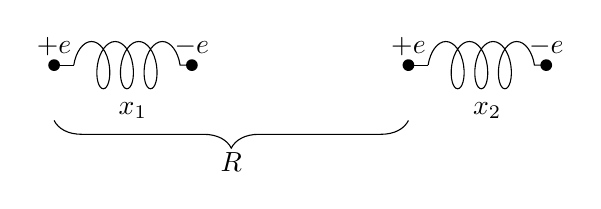
\begin{tikzpicture}
\draw[decoration={aspect=0.5, segment length=3mm, amplitude=3mm,coil},decorate] (0,0) --++ (1.5,0) node[fill=black,inner sep=1.5pt, circle]{} node[above]{$-e$} node[pos=0.5, below,yshift=-1em]{$x_1$};
\draw[] (0,0) --++ (-0.25,0) node[fill=black,inner sep=1.5pt,circle]{} node[above]{$+e$};
\draw[decoration={aspect=0.5, segment length=3mm, amplitude=3mm,coil},decorate] (4.5,0) --++ (1.5,0) node[fill=black,inner sep=1.5pt, circle]{} node[above]{$-e$} node[pos=0.5, below,yshift=-1em]{$x_2$};
\draw[] (4.5,0) --++ (-0.25,0) node[fill=black,inner sep=1.5pt,circle]{} node[above]{$+e$};
\draw[decorate,decoration={brace,amplitude=10pt,mirror},yshift=-20pt] (-0.25,0) -- (4.25,0) node[midway,yshift=-15pt]{$R$};
\end{tikzpicture}
\caption{
دو  قابل تقطیب  قریبی جوہر (سوال \حوالہء{6.31})۔
}
\label{
شکل_غیر_تابع_اضطراب_قابل_تقطیب
}
\end{figure}



%===================================

%fig 6.15 pg 303

\begin{figure}
\centering
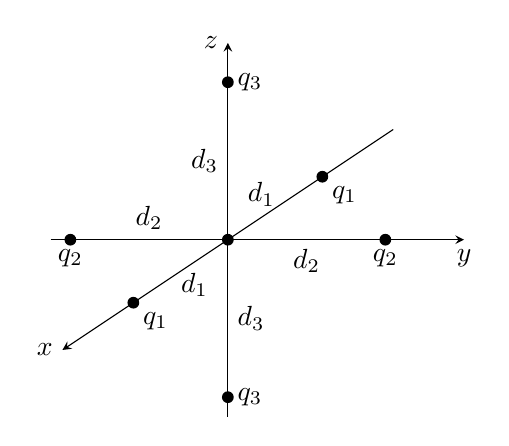
\begin{tikzpicture}[x={(-0.6cm,-0.4cm)},y={(1cm,0cm)},z={(0cm,1cm)}]
\draw[-stealth](0,-2.25,0) -- (0,3,0) node[below]{$y$};
\draw[-stealth](-3.5,0,0) -- (3.5,0,0) node[left]{$x$};
\draw[-stealth](0,0,-2.25) -- (0,0,2.5) node[left]{$z$};
\draw[](-2,0,0) node[fill=black,inner sep=1.5pt,circle]{} node[below right]{$q_1$};
\draw[](2,0,0) node[fill=black,inner sep=1.5pt,circle]{} node[below right]{$q_1$};
\draw[](0,-2,0) node[fill=black,inner sep=1.5pt,circle]{} node[below]{$q_2$};
\draw[](0,2,0) node[fill=black,inner sep=1.5pt,circle]{} node[below]{$q_2$};
\draw[](0,0,-2) node[fill=black,inner sep=1.5pt,circle]{} node[right]{$q_3$};
\draw[](0,0,2) node[fill=black,inner sep=1.5pt,circle]{} node[right]{$q_3$};
\draw[] (-1,0,0) node[shift={(-5pt,5pt)}]{$d_1$};
\draw[] (1,0,0) node[shift={(5pt,-5pt)}]{$d_1$};
\draw[] (0,-1,0) node[above]{$d_2$};
\draw[] (0,1,0) node[below]{$d_2$};
\draw[] (0,0,-1) node[right]{$d_3$};
\draw[] (0,0,1) node[left]{$d_3$};
\draw(0,0,0) node[circle,fill=black,inner sep=1.5pt]{};
\end{tikzpicture}
\caption{
ہائیڈروجن جوہر کے گرد   چھ نقطی بار (قلمی جال کا ایک سادہ نمونہ)؛ سوال \حوالہء{6.39}
}
\label{
شکل_غیر_تابع_اضطراب_قلمی_جال
}
\end{figure}



%===================================

%fig 7.1 pg 308

\begin{figure}
\centering
\begin{tikzpicture}
\fill[path fading=west,color=lgray] (-0.25,0) rectangle (0,3.75);
\fill[path fading=east,color=lgray] (5,0) rectangle (5.25,3.75);
\draw[-stealth] (-0.5,0) -- (5.75,0)node[below]{$x$};
\draw[-stealth] (0,-0.25) -- (0,4)node[left]{$\psi(x)$};
\draw[very thick](0,0) -- (2.5,3) -- (5,0) node[below]{$a$};
\draw[](2.5,0.1) -- (2.5,-0.1) node[below]{$a/2$};
\draw[](5,0) -- (5,3.75);
\end{tikzpicture}
\caption{
لامتناہی چکور کنواں کے لئے تکونی تفاعل موج (مساوات \حوالہء{7.10})۔
}
\label{
شکل_تغیریت_لامتناہی_کنواں_تکونی_موج
}
\end{figure}



%===================================

%fig 7.2 pg 309

\begin{figure}
\centering
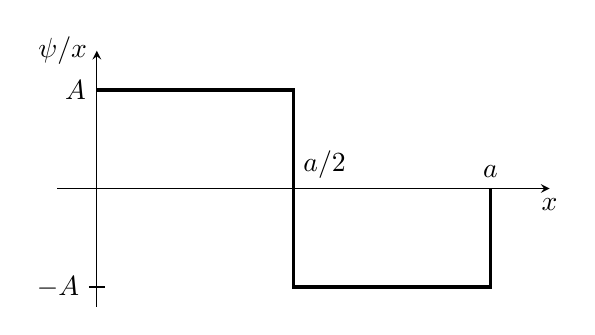
\begin{tikzpicture}
\draw[-stealth] (-0.5,0) -- (5.75,0)node[below]{$x$};
\draw[-stealth] (0,-1.5) -- (0,1.75)node[left]{$\dif\psi/\dif x$};
\draw[very thick](0,1.25) node[left]{$A$} -- (2.5,1.25) -- (2.5,-1.25) -- (5,-1.25) -- (5,0) node[above]{$a$};
\draw[] (-0.1,-1.25) node[left]{$-A$} -- (0.1,-1.25);
\draw[] (2.5,0) node[above right]{$a/2$};
\end{tikzpicture}
\caption{
لامتناہی چکور کنواں میں تکونی تفاعل موج (شکل \حوالہء{7.1}) کا تفرق۔
}
\label{
شکل_تغیریت_لامتناہی_کنواں_تکونی_موج_تفرق
}
\end{figure}



%===================================

%fig 7.3 pg 311

\begin{figure}
\centering
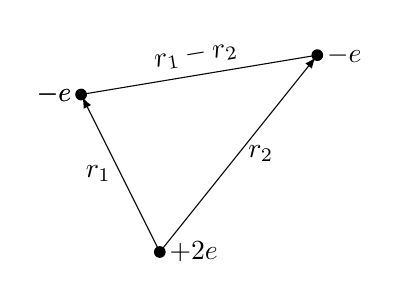
\begin{tikzpicture}
\draw[-latex,shorten >=1pt] (0,0) node[right]{$+2e$} node[circle, fill=black,inner sep=1.5pt]{} -- (-1,2) node[left]{$-e$} node[pos=0.5,left]{$\kvec{r}_1$};
\draw[] (-1,2) node[left]{$-e$} node[circle, fill=black,inner sep=1.5pt]{} -- (2,2.5) node[right]{$-e$} node[pos=0.5,above,sloped]{$\abs{\kvec{r}_1-\kvec{r}_2}$} node[circle, fill=black,inner sep=1.5pt]{};
\draw[-latex,shorten >=1pt] (0,0) -- (2,2.5) node[pos=0.5,right]{$\kvec{r}_2$};
\end{tikzpicture}
\caption{
ہیلیم جوہر۔
}
\label{
شکل_تغیریت_ہیلیم_جوہر
}
\end{figure}



%===================================

%fig 7.4 pg 313

\begin{figure}
\centering
\begin{tikzpicture}[x={(-0.5cm,-0.5cm)}, y={(1cm,0cm)}, z={(0cm,1cm)}]
\pgfmathsetmacro{\p}{atan(2/0.5)}
\pgfmathsetmacro{\t}{acos(2.5/sqrt(0.5^2+2^2+2.5^2))}
\draw[-stealth] (0,0,0) -- (1.5,0,0) node[left]{$x_2$};
\draw[-stealth] (0,0,0) -- (0,3,0) node[below]{$y_2$};
\draw[-stealth] (0,0,0) -- (0,0,3) node[left]{$z_2$};
\draw[very thick, -latex,shorten >=1pt] (0,0,0) node[circle, fill=black,inner sep=1.5pt]{} -- (0,0,2) node[pos=0.75,left]{$\kvec{r}_1$};
\draw[very thick] (0,0,2) node[circle, fill=black,inner sep=1.5pt]{} -- (0.5, 2, 2.5) node[pos=0.5,above,sloped]{$\abs{\kvec{r}_1-\kvec{r}_2}$} node[circle, fill=black,inner sep=1.5pt]{};
\draw[very thick, -latex,shorten >=1pt] (0,0,0) -- (0.5,2,2.5) node[pos=0.5,right]{$\kvec{r}_2$};
\draw[dashed] (0,0,0) -- (0.5,2,0) -- (0.5,2,2.5);
\begin{scope}[canvas is xy plane at z=0]
\draw[-stealth] ([shift=(0:0.75)]0,0,0) arc (0:75:0.75)node[pos=0.5,below right]{$\phi_2$};
\end{scope}
\draw[-stealth,domain=0:\t] plot ({1*sin(\x)*cos(\p)},{1*sin(\x)*sin(\p)},{cos(\x)});
\draw(0,0.4,0.8)node[above]{$\theta_2$};
\end{tikzpicture}
\caption{
محدد کا انتخاب برائے \عددی{\kvec{r}_2} تکمل (مساوات \حوالہء{7.20})۔
}
\label{
شکل_تغیریت_محدد_انتخاب_رداس_دوم_تکمل
}
\end{figure}


%===================================

%fig 7.5 pg 316

\begin{figure}
\centering
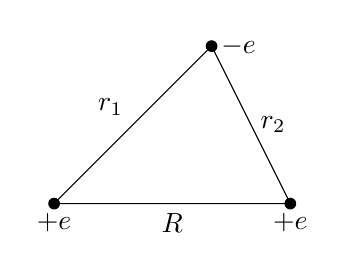
\begin{tikzpicture}
\draw[] (0,0) node[below]{$+e$} node[circle, fill=black,inner sep=1.5pt]{} -- (3,0) node[pos=0.5, below]{$R$} node[below]{$+e$} node[circle, fill=black,inner sep=1.5pt]{} -- (2,2) node[pos=0.5, right]{$r_2$} node[right]{$-e$} node[circle, fill=black,inner sep=1.5pt]{} -- (0,0) node[pos=0.5, above left]{$r_1$};
\end{tikzpicture}
\caption{
ہائیڈروجن سالمہ بارداریہ، \عددی{
\ce{H}_2^+
}
}
\label{
شکل_تغیریت_ہائیڈروجن_سالمہ_بارداریہ
}
\end{figure}



%=====



%===================================

%fig 7.6 pg 317

\begin{figure}
\centering
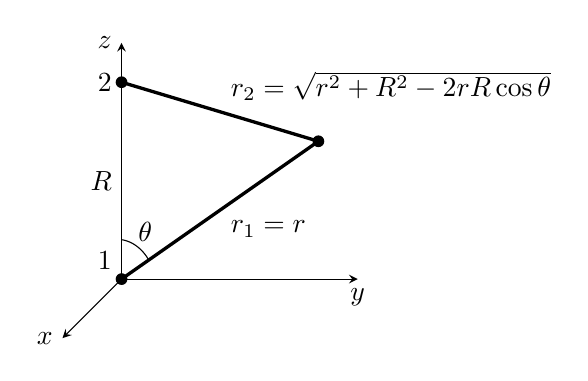
\begin{tikzpicture}[x={(-0.5cm,-0.5cm)}, y={(1cm,0cm)}, z={(0cm,1cm)}]
\pgfmathsetmacro{\p}{atan(2/0.5)}
\pgfmathsetmacro{\t}{acos(2/sqrt(0.5^2+2.75^2+2^2))}
\draw[-stealth] (0,0,0) -- (1.5,0,0) node[left]{$x$};
\draw[-stealth] (0,0,0) -- (0,3,0) node[below]{$y$};
\draw[-stealth] (0,0,0) -- (0,0,3) node[left]{$z$};
\draw[] (0,0,0) node[above left]{$1$} node[circle, fill=black,inner sep=1.5pt]{} -- (0,0,2.5) node[left]{$2$} node[pos=0.5,left]{$R$};
\draw[very thick] (0,0,2.5) node[circle, fill=black,inner sep=1.5pt]{} -- (0.5, 2.75, 2) node[pos=0.5,above right]{$r_2=\sqrt{r^2 + R^2 -2rR\cos \theta}$} node[circle, fill=black,inner sep=1.5pt]{};
\draw[very thick] (0,0,0) -- (0.5,2.75,2) node[pos=0.5,below right]{$r_1=r$};
\draw[domain=0:\t] plot ({0.5*sin(\x)*cos(\p)},{0.5*sin(\x)*sin(\p)},{0.5*cos(\x)});
\draw(0,0.3,0.6)node[]{$\theta$};
\end{tikzpicture}
\caption{
مقدار \عددی{I} کے حساب کی خاطر محدد (مساوات \حوالہء{7.39})۔
}
\label{
شکل_تغیریت_محدد_قدار_آئے
}
\end{figure}




%======================
%fig 7.7 page 320


\begin{figure}
\centering
\begin{tikzpicture}[declare function={fa(\x)=(1-2/3*\x^2)*e^(-\x); fb(\x)=(1+\x)*e^(-2*\x); fc(\x)=1+(1+\x+1/3*\x^2)*e^(-\x); f(\x)=-1+2*(fa(\x)+fb(\x))/(\x*fc(\x));}]
\begin{axis}[axis lines=middle,axis x line shift=1,xlabel={$x$},ylabel={$F(x)$}, xtick={1,2,2.25,3,4,5,6}, xticklabels={$1$,$2$,,$3$,$4$,$5$,$6$}, ytick={-1.2,-1,-0.5,0}, ylabel style={at={(current axis.above origin)},anchor=east},,enlargelimits,ymax=0,ymin=-1.3]
\addplot [thick,domain=0.7:6,smooth] {f(x)};
\addplot[] coordinates{(2.25,-1)} node[pin={45:{توازن}}]{};
\end{axis}
\end{tikzpicture}
\caption{
تفاعل \عددی{F(x)} (مساوات \حوالہء{7.51})  کی ترسیم  مقید حال کی موجودگی دکھاتی ہے (بوہر رداس کی اکائیوں میں \عددی{x} دو پروٹانوں کے بیچ فاصلہ ہے)۔ 
}
\label{
شکل_تغیریت_مقید_حال
}
\end{figure}


%===================================

%fig 7.8 pg 326

\begin{figure}
\centering
\begin{tikzpicture}
\draw[-stealth] (-3,0) -- (3.25,0) node[below]{$x$};
\draw[-stealth] (0,-2) -- (0,2.25) node[left]{$y$};
\fill[,color=lgray] (-3,-1) rectangle (-1,-2);
\fill[,color=lgray] (-3,1) rectangle (-1,2);
\fill[,color=lgray] (3,-1) rectangle (1,-2);
\fill[,color=lgray] (3,1) rectangle (1,2);
\draw[thick] (-3,-1) -- (-1,-1) -- (-1,-2);
\draw[thick] (-3,+1) -- (-1,+1) -- (-1,+2);
\draw[thick] (3,-1) -- (1,-1) -- (1,-2);
\draw[thick] (3,1) -- (1,1) -- (1,2);
\draw[](-0.1,1) -- (0.1,1) node[right]{$a$};
\draw[](-0.1,-1) -- (0.1,-1) node[right]{$-a$};
\draw[](-1,0.1) -- (-1,-0.1) node[below]{$-a$};
\draw[](1,0.1) -- (1,-0.1) node[below]{$a$};
\end{tikzpicture}
\caption{
صلیبی  خطہ برائے سوال \حوالہء{7.20}
}
\label{
شکل_تغیریت_صلیبی_خطہ
}
\end{figure}



%===================================

%fig 8.1 pg 329

\begin{figure}
\centering
\begin{tikzpicture}
\draw[-stealth] (-0.25,0) -- (5.25,0) node[below]{$x$};
\draw[-stealth] (0,-0.15) -- (0,2.5) node[left]{$V(x)$};
\draw[thick,name path=a](0.25,2.25) to [out=-5,in=180] (2.5,0.5) to [out=0,in=-150] (5,2);
\draw[dashed,name path=b] (0,1.75) node[left]{$E$} -- (5,1.75);
\draw[dashed,name intersections={of=a and b}] (intersection-1) node[pin={[pin edge={-,solid},pin distance=1cm]45:{\RL{نقاط واپسیں}}}]{} -- ($(0,0)!(intersection-1)!(5,0)$)coordinate(c);
\draw[dashed,name intersections={of=a and b}] (intersection-2)node[pin={[pin edge={-,solid},pin distance=1cm]135:{}}]{} -- ($(0,0)!(intersection-2)!(5,0)$)coordinate(d);
\draw[decorate,decoration={brace,amplitude=10pt, mirror},yshift=-10pt] ($(c)+(0,-0.1)$) -- ($(d)+(0,-0.1)$) node[midway,below,yshift=-7pt]{\RL{کلاسیکی خطہ}};
\end{tikzpicture}
\caption{
کلاسیکی طور پر یہ ذرہ اس خطہ میں مقید ہو گا جہاں \عددی{E\ge V(x)} ہو ۔
}
\label{
شکل_وکب_کلاسیکی_مقید_خطہ
}
\end{figure}


%===================================

%fig 8.2 pg 330

\begin{figure}
\centering
\begin{tikzpicture}
\fill[path fading=west,color=lgray] (-0.25,0) rectangle (0,3.75);
\fill[path fading=east,color=lgray] (5,0) rectangle (5.25,3.75);
\draw[-stealth] (-0.5,0) -- (5.75,0)node[below]{$x$};
\draw[-stealth] (0,-0.25) -- (0,4)node[left]{$V(x)$};
\draw[very thick](0,3.75) -- (0,1) to [out=30,in=180] (2,0.5) to [out=0,in=180] (3,0.75) to [out=0,in=180] (5,0.25) -- (5,3.75); \draw (5,0) node[below]{$a$};
\draw[](5,0) -- (5,3.75);
\end{tikzpicture}
\caption{
ایسا لامتناہی چکورکنواں جس کی تہہ موڑےدار ہو۔
}
\label{
شکل_وکب_لامتناہی_موڑا
}
\end{figure}



%===================================

%fig 8.3 pg 333

\begin{figure}
\centering
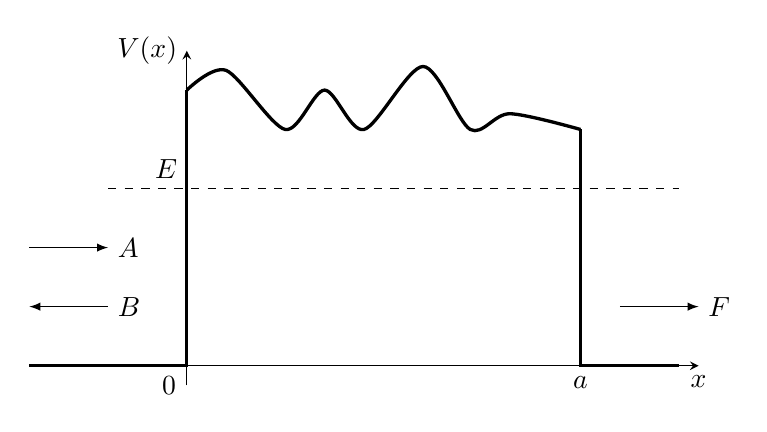
\begin{tikzpicture}
\draw[-stealth] (-0.5,0) -- (6.5,0)node[below]{$x$};
\draw[-stealth] (0,-0.25) -- (0,4)node[left]{$V(x)$};
%\draw[very thick](-2,0) -- (0,0) -- (0,3) to [out=30,in=180] ++(0.5,0) to [out=0,in=180] ++(0.75,-0.25) to [out=0,in=180] +%+(1,0.5) to [out=0,in=180] (5,3.5) -- (5,0)node[below]{$a$}-- (6,0);
\draw[very thick](-2,0) -- (0,0) node[below left]{$0$}-- (0,3.5) (5,3)--(5,0)node[below]{$a$}--(6.25,0);
\draw[very thick] plot [smooth] coordinates {(0,3.5)(0.5,3.75)(1.25,3)(1.75,3.5)(2.25,3)(3,3.8)(3.6,3)(4.1,3.2)(5,3)};
\draw[dashed](-1,2.25)--(6.25,2.25);
\draw[-latex](-2,1.5)--++(1,0)node[right]{$A$};
\draw[latex-](-2,0.75)--++(1,0)node[right]{$B$};
\draw[-latex](5.5,0.75)--++(1,0)node[right]{$F$};
\draw(0,2.25)node[above left]{$E$};
\end{tikzpicture}
\caption{
موڑے دار بالائی سطح کے   مستطیلی رکاوٹ سے بکھراو۔
}
\label{
شکل_وکب_مستطیلی_رکاوٹ
}
\end{figure}




%===================================

%fig 8.4 pg 334

\begin{figure}
\centering
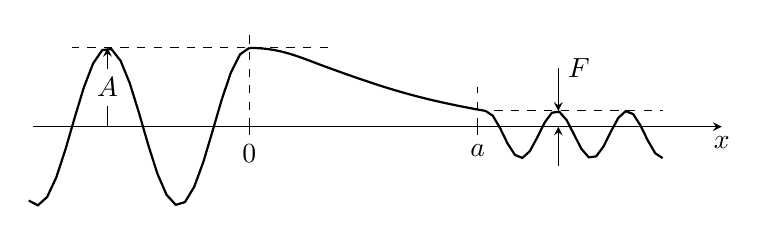
\begin{tikzpicture}
\draw[-stealth] (-2.75,0) -- (6,0)node[below]{$x$};
%\draw[-stealth] (0,-0.25) -- (0,4)node[left]{$V(x)$};
\draw[-stealth](-360/200,0) -- (-360/200,1) node[pos=0.5, fill=white]{$A$};
\draw[thick,domain=-560:0] plot ({\x/200},{cos(\x)});
\draw[thick,smooth](0,1) to [out = 0,in=160] ++ (1,-0.25) to [out=-20,in=170] ++ (2,-0.55);
\draw[thick,domain=0:900] plot ({3+\x/400},{-0.1+0.3*cos(\x)});
\draw[dashed](0,0) -- (0,1.25) (1,1) -- (-2.25,1); 
\draw[](0,0.1)--++(0,-0.2) node[below]{$0$};
\draw[dashed](2.9,0) -- (2.9,0.5) (2.9,0.2) -- (5.25,0.2); 
\draw[](2.9,0.1)--++(0,-0.2) node[below]{$a$};
\draw[-stealth] (3.925,-0.5) -- (3.925,0);
\draw[stealth-] (3.925,0.2) -- (3.925,0.75) node[right]{$F$};
\end{tikzpicture}
\caption{
اونچی اور چوڑی رکاوٹ سے بکھراو کے تفاعل  موج کی کیفی ساخت۔
}
\label{
شکل_وکب_اونچی_چوڑی
}
\end{figure}


%==================================


%fig 8.5 pg 335

\begin{figure}
\centering
\begin{tikzpicture}[declare function={f(\x)= 1/(\x);}]
\pgfmathsetmacro{\E}{f(4)}
\begin{axis}[axis lines=middle,xlabel={$r$},ylabel={$V(r)$}, xtick={1,4},
 xticklabels={\rlap{$r_1$} ,$r_2$, $0$}, ytick={-0.5,\E}, yticklabels={$-V_0$,$E$}, ylabel style={at={(current axis.above origin)},anchor=east},xlabel style={at={(current axis.right of origin)},anchor=north east},enlargelimits]
\addplot [thick,domain=1:5]{f(x)}node[pos=0.5,pin={45:{\RL{کولمب دفع}}}]{};
\addplot[thick,]coordinates{({1},{f(1)})(1,-0.5)(0,-0.5)};
\addplot[thick,]coordinates{(0,\E)(5,\E)};
\addplot[]coordinates{(0.75,-0.5)}node[pin={45:{\RL{مرکزوی بندش}}}]{};
\end{axis}
\end{tikzpicture}
\caption{
تابکار مرکزی میں الفا ذرہ کی مخفی توانائی کا گامو نمونہ۔
}
\label{
شکل_وکب_گامو_نمونہ
}
\end{figure}



%==================================


%fig 8.7 pg 338

\begin{figure}
\centering
\begin{tikzpicture}
\fill[lgray] (-1,0.5) rectangle (1,3.75);
\draw[-stealth](-3,-0.5) -- (3.5,-0.5) node[below]{$x$};
\draw[-stealth](0,-0.75) -- (0,4) node[left]{$V(x)$};
\draw[] (-2.75,2.125) -- (2.75,2.125) node[right]{$E$};
\draw[name path=a,decoration={random steps,segment length=0.5mm,amplitude=0.5pt},decorate](-1,0.5) -- (-1,3.75);
\draw[name path=b,decoration={random steps,segment length=0.5mm,amplitude=0.5pt},decorate](1,0.5) -- (1,3.75);
\draw[decoration={brace,amplitude=5pt,raise=4pt, mirror},decorate] (-1,0.5) -- (1,0.5) node[midway,below left,yshift=-12pt]{\RL{پیوندکار خطہ}};
\draw[](0,2.125) node[pin={[pin distance=1.25cm]135:{\RL{نقطہ واپسیں}}}]{} --++ (45:2) node[pos=1,pin={10:{\RL{خط بند مخفیہ}}}]{};
\draw[](0,2.125) --++ (-135:2);
\draw[thick] (0,2.125) to [out=45,in=180] (2,3);
\draw[thick] (0,2.125) to [out=-135,in=0] (-2,1.25);
\draw[] (-2,-0.75) -- (-0.25,-0.75) node[pos=0.5,below]{\RL{کلاسیکی خطہ}}; 
\draw[] (+2,-0.75) -- (+0.25,-0.75) node[pos=0.5,below]{\RL{غیر کلاسیکی خطہ}}; 
\end{tikzpicture}
\caption{
دائیں ہاتھ نقطہ واپسیں کو  وضاحت سے دکھایا گیا ہے۔
}
\label{
شکل_وکب_نقطہ_واپسیں_وضاحت
}
\end{figure}


%==================================


%fig 8.9 pg 341

\begin{figure}
\centering
\begin{tikzpicture}
\fill[lgray] (-2.5,0.5) rectangle (-1.5,3.75);
\fill[lgray] (1.5,0.5) rectangle (2.5,3.75);
\draw[-stealth](-3,0.5) -- (3.5,0.5) node[below]{$x$};
\draw[](0,-0.65) -- (0,4);
\draw[name path=a,decoration={random steps,segment length=0.5mm,amplitude=0.5pt},decorate](-2.5,0.5) -- (-2.5,3.75);
\draw[name path=b,decoration={random steps,segment length=0.5mm,amplitude=0.5pt},decorate](-1.5,0.5) -- (-1.5,3.75);
\draw[name path=a,decoration={random steps,segment length=0.5mm,amplitude=0.5pt},decorate](2.5,0.5) -- (2.5,3.75);
\draw[name path=b,decoration={random steps,segment length=0.5mm,amplitude=0.5pt},decorate](1.5,0.5) -- (1.5,3.75);
\draw[decoration={brace,amplitude=5pt,raise=4pt, mirror},decorate] (-2.5,0.5) -- (-1.5,0.5) node[midway,below,yshift=-12pt]{\RL{جزوی منطبق خطہ}};
\draw[decoration={brace,amplitude=5pt,raise=4pt, mirror},decorate] (1.5,0.5) -- (2.5,0.5) node[midway,below,yshift=-12pt]{\RL{جزوی منطبق خطہ}};
\draw[] (-2.5,-0.75) -- (2.5,-0.75) node[pos=0.5,below]{\RL{پیوندکار خطہ}};
\draw[](0,0.5) node[fill=black,circle,inner sep=1.5pt]{} node[pin={[text centered, text width=1cm]45:{\RL{نقطہ واپسیں}}}]{};
\draw[stealth-stealth] (-2.5,2.5) -- (2.5,2.5) node[pos=0.6,fill=white]{$\psi_p$};
\draw[stealth-] (-1.5,3) -- (-3.75,3) node[above right]{$\psi_{WKB}$};
\draw[stealth-] (1.5,3) -- (3.75,3) node[above left]{$\psi_{WKB}$};
\end{tikzpicture}
\caption{
پیوندکار خطہ اور دو  منطبق  خطے۔
}
\label{
شکل_وکب_پیوندکار_منطبق
}
\end{figure}


%===================================

%fig 8.10 pg 343

\begin{figure}
\centering
\begin{tikzpicture}
\fill[path fading=west,color=lgray] (-0.25,0) rectangle (0,3.75);
\draw[-stealth] (-0.5,0) -- (5.75,0)node[below]{$x$};
\draw[-stealth] (0,-0.25) -- (0,4)node[left]{$V(x)$};
\draw[very thick, name path=a] (0,3.5) -- (0,0.25) to [out=0,in=180] ++ (2,1) to [out=0,in=-120] ++ (2,1) to [out=60,in=-160] ++ (1,1); 
\draw[name path=b](0,2) node[left,xshift={-0.5em}]{$E$} -- (5,2);
\draw[dashed,name intersections={of={a and b}}] (intersection-2) -- ($(0,0)!(intersection-2)!(5,0)$) node[below]{$x_2$};
\end{tikzpicture}
\caption{
ایک  ایتصابی  دیوار والا مخفیہ کنواں۔
}
\label{
شکل_وکب_ایک_دیوار_کنواں
}
\end{figure}




%===================================

%fig 8.11 pg 344

\begin{figure}
\centering
\begin{subfigure}{0.22\textwidth}
\centering 
\pgfmathsetmacro{\a}{70}
\pgfmathsetmacro{\b}{180-\a}
\begin{tikzpicture}
%\draw[-stealth] (0,0) -- (0.5,0)node[below]{$x$};
%\draw[-stealth] (0,0) -- (0,3)node[left]{$V(x)$};
\draw[] (-1,0) node[left]{$E$} -- (1,0);
\draw[dashed] (0,-1) node[below]{$x_2$} -- (0,1);
\draw[very thick, name path=a] (0,0) to [out=\a,in=-170] ++ (1,1); 
\draw[very thick, name path=a] (0,0) to [out=-\b,in=10] ++ (-1,-1); 
\end{tikzpicture}
\caption{}
\end{subfigure}\hfill
\begin{subfigure}{0.22\textwidth}
\centering 
\pgfmathsetmacro{\a}{70}
\pgfmathsetmacro{\b}{180-\a}
\begin{tikzpicture}
%\draw[-stealth] (0,0) -- (0.5,0)node[below]{$x$};
%\draw[-stealth] (0,0) -- (0,3)node[left]{$V(x)$};
\draw[] (-1,0) node[left]{$E$} -- (1,0);
\draw[dashed] (0,-1) node[below]{$x_1$} -- (0,1);
\draw[very thick, name path=a] (0,0) to [out=-\a,in=170] ++ (1,-1); 
\draw[very thick, name path=a] (0,0) to [out=\b,in=-10] ++ (-1,1); 
\end{tikzpicture}
\caption{}
\end{subfigure}\hfill
\begin{subfigure}{0.45\textwidth}
\centering 
\pgfmathsetmacro{\a}{70}
\pgfmathsetmacro{\b}{180-\a}
\begin{tikzpicture}
\draw[-stealth] (-1.5,-1.5) -- ++(0.5,0)node[below]{$x$};
\draw[-stealth] (-1.5,-1.5) -- ++(0,3)node[below left]{$V(x)$};
\draw[] (-1,0) node[left]{$E$} -- (3,0);
\draw[dashed] (0,-1) node[below]{$x_1$} -- (0,1);
\draw[dashed] (2,-1) node[below]{$x_2$} -- (2,1);
\draw[very thick, name path=a] (0,0) to [out=-\a,in=180] ++ (1,-1); 
\draw[very thick, name path=a] (0,0) to [out=\b,in=-10] ++ (-1,1); 
\draw[very thick, name path=a] (2,0) to [out=-\b,in=0] ++ (-1,-1); 
\draw[very thick, name path=a] (2,0) to [out=\a,in=-170] ++ (1,1); 
\end{tikzpicture}
\caption{}
\end{subfigure}
\caption{
بالائی جانب ڈھلوان اور نیچے جانب ڈھلون نقطہ وپسیں۔
}
\label{
شکل_وکب_بالائی_جانب_نقطہ_واپسیں
}
\end{figure}




%==============================


%fig 8.12 pg 347

\begin{figure}
\centering 
\begin{tikzpicture}
\pgfmathsetmacro{\a}{135}
\pgfmathsetmacro{\b}{180 - \a}
\draw[-stealth] (-3,0) -- (3,0)node[below]{$x$};
\draw[-stealth] (0,-0.25) -- (0,3)node[left]{$V(x)$};
\draw[name path=a] (-3,1.5) node[left]{$E$} -- (3,1.5);
\draw[very thick, name path=b] (-3,0.2) to [out=10,in=-\a] ++ (2,2) to [out=\b, in=0] (0,2.5) to [out=0,in=-180] ++ (0.5,0.25) to [out=0,in=170] (3,0.2);
\draw[dashed,name intersections={of={a and b}}] (intersection-1) -- ($(-3,0)!(intersection-1)!(3,0)$) node[below]{$x_1$}  (intersection-1) --++ (0,0.25);
\draw[dashed,name intersections={of={a and b}}] (intersection-2) -- ($(-3,0)!(intersection-2)!(3,0)$) node[below]{$x_2$}  (intersection-2) --++ (0,0.25);
\end{tikzpicture}
\caption{
ڈھلوانی دیواروں والا رکاوٹ۔
}
\label{
شکل_وکب_ڈھلوانی_دیواروں_رکاوٹ
}
\end{figure}


%==============================


%fig 8.13 pg 349

\begin{figure}
\centering 
\begin{tikzpicture}
\pgfmathsetmacro{\a}{135}
\pgfmathsetmacro{\b}{180 - \a}
\draw[-stealth] (-3,0) -- (3.5,0)node[below]{$x$};
\draw[-stealth] (0,-0.25) -- (0,3)node[left]{$V(x)$};
\draw[name path=a] (-3,1) node[left]{$E$} -- (3,1);
\draw[very thick, name path=b] (0,1.5) to [out=0,in=180] (1,0) to [out=0, in=-100] (3,2.5)  (0,1.5) to [out=180,in=0] (-1,0) to [out=180, in=-90] (-3,2.5);
\draw[dashed,name intersections={of={a and b}}] (intersection-1) -- ($(-3,0)!(intersection-1)!(3,0)$) node[below]{$x_1$}  (intersection-1) --++ (0,0.25);
\draw[dashed,name intersections={of={a and b}}] (intersection-2) -- ($(-3,0)!(intersection-2)!(3,0)$) node[below]{$x_2$}  (intersection-2) --++ (0,0.25);
\end{tikzpicture}
\caption{
تشاکلی دہرا کنواں؛ سوال \حوالہء{8.15}۔
}
\label{
شکل_وکب_تشاکلی_دہرا_کنواں
}
\end{figure}


%==============================


%fig 9.1 pg 359

\begin{figure}
\centering
\begin{tikzpicture}[declare function={f(\x)= 1-cos(\x);}]
\begin{axis}[axis lines=middle,xlabel={$t$},ylabel={$P(t)$}, xtick={360,720,1080},
 xticklabels={$\tfrac{2\pi}{\abs{\omega_0-\omega}}$ ,$\tfrac{4\pi}{\abs{\omega_0-\omega}}$, $\tfrac{6\pi}{\abs{\omega_0-\omega}}$}, ytick={2}, yticklabels={$\abs{\tfrac{\abs{V_{ab}}}{\hslash(\omega_0-\omega)}}^2$}, ylabel style={at={(current axis.above origin)},anchor=west},xlabel style={at={(current axis.right of origin)},anchor=north east},enlargelimits]
\addplot [thick,smooth,domain=0:1260]{f(x)};
\addplot [dashed] coordinates{(0,2)(1260,2)};
\end{axis}
\end{tikzpicture}
\caption{
سائن نما اضطراب کے لئے وقت کے لحاظ سے تحویلی احتمال (مساوات \حوالہء{9.28})۔
}
\label{
شکل_تابع_وقت_احتمال_سائن_نما_احتمال
}
\end{figure}


%==============================


%fig 9.2 pg 359

\begin{figure}
\centering
\pgfmathsetmacro{\k}{15}
\pgfmathsetmacro{\ka}{\k-2*pi}
\pgfmathsetmacro{\kb}{\k+2*pi}
\begin{tikzpicture}[declare function={f(\x)= (sin(deg(\k-\x)/2)^2)/pow(\k-\x,2);}]
\begin{axis}[clip=false,axis lines=middle,xlabel={$\omega$},ylabel={$P(\omega)$}, xtick={\k,\ka,\kb},
 xticklabels={$\omega_0$,,}, ytick={0.25}, yticklabels={}, ylabel style={at={(current axis.above origin)},anchor= east},xlabel style={at={(current axis.right of origin)},anchor=north east},enlargelimits]
\addplot [thick,smooth,domain=0:30,samples=50]{f(x)};
\addplot[] coordinates {(\ka,0)}node[pin=-120:{$(\omega_0-2\pi/t)$}]{};
\addplot[] coordinates {(\kb,0)}node[pin=-60:{$(\omega_0+2\pi/t)$}]{};
\end{axis}
\end{tikzpicture}
\caption{
تحویلی احتمال بالمقابل   متحرک  تعدد  (مساوات \حوالہء{9.28})۔
}
\label{
شکل_تابع_وقت_احتمال_جبری_تعدد
}
\end{figure}



